\documentclass[tikz, border=1pt]{standalone}
\usepackage{tikz}
\usetikzlibrary{arrows.meta, positioning}
\usepackage{xcolor,colortbl}
% Define extra colors
\definecolor{darkgreen}{rgb}{0.0, 0.5, 0.0} % Define a darker green

\begin{document}

\begin{figure}
    \centering

    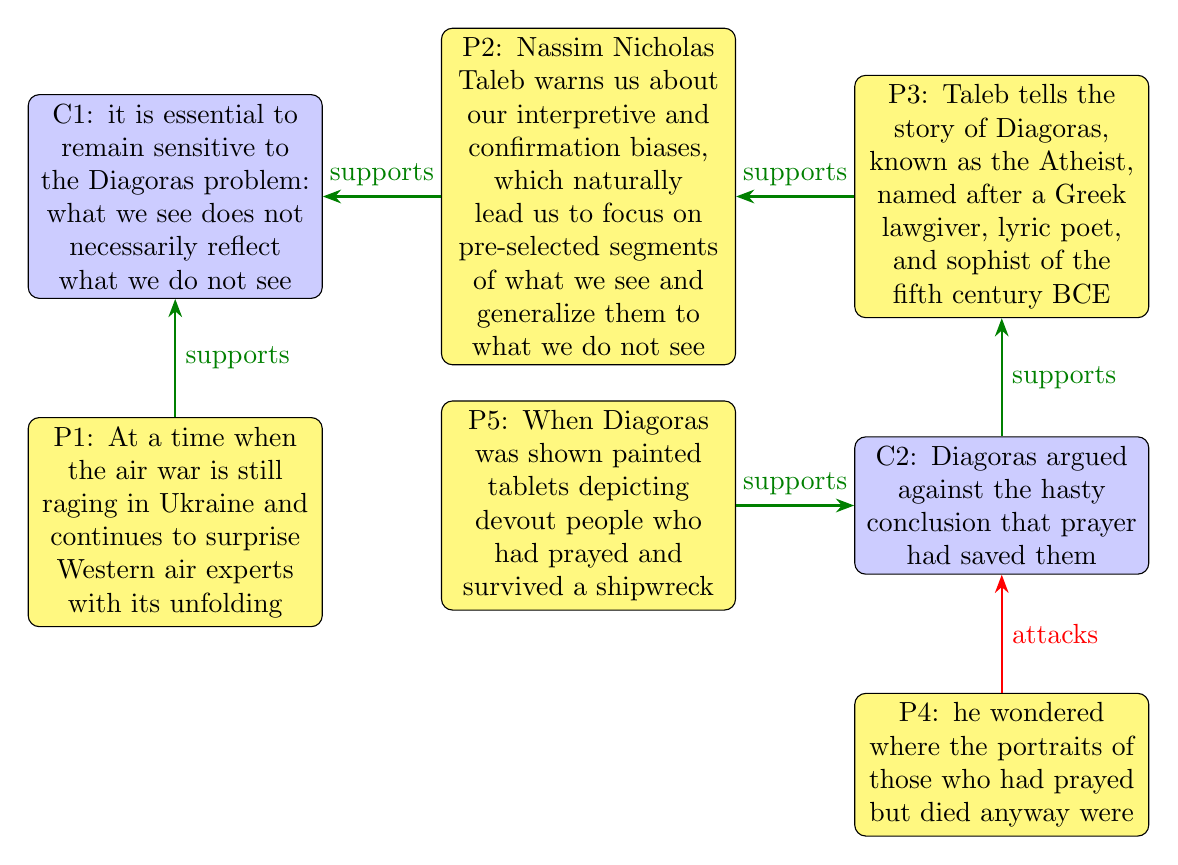
\begin{tikzpicture}[
        claim/.style={rectangle, draw, rounded corners, align=center, text width=3.5cm, minimum height=1.5cm, fill=blue!20},
        premise/.style={rectangle, draw, rounded corners, align=center, text width=3.5cm, minimum height=1.5cm, fill=yellow!50},
        arrow/.style={-{Stealth}, thick},
        support/.style={draw, -{Stealth}, thick, darkgreen},
        attack/.style={draw, -{Stealth}, thick, red},
        node distance=1.5cm and 1.5cm
        ]

        % Nodes
        \node (claim1) [claim] {C1: it is essential to remain sensitive to the Diagoras problem: what we see does not necessarily reflect what we do not see};
        \node (premise2) [premise, right=of claim1] {P2: Nassim Nicholas Taleb warns us about our interpretive and confirmation biases, which naturally lead us to focus on pre-selected segments of what we see and generalize them to what we do not see};
        \node (premise3) [premise, right=of premise2] {P3: Taleb tells the story of Diagoras, known as the Atheist, named after a Greek lawgiver, lyric poet, and sophist of the fifth century BCE};
        \node (premise1) [premise, below=of claim1] {P1: At a time when the air war is still raging in Ukraine and continues to surprise Western air experts with its unfolding};
        \node (claim2) [claim, below=of premise3] {C2: Diagoras argued against the hasty conclusion that prayer had saved them};
        \node (premise4) [premise, below=of claim2] {P4: he wondered where the portraits of those who had prayed but died anyway were};
        \node (premise5) [premise, left=of claim2] {P5: When Diagoras was shown painted tablets depicting devout people who had prayed and survived a shipwreck};

        % Arrows with labels
        \draw [support] (premise1) -- node[midway, right] {supports} (claim1);
        \draw [support] (premise2) -- node[midway, above] {supports} (claim1);
        \draw [support] (premise3) -- node[midway, above] {supports} (premise2);
        \draw [support] (claim2) -- node[midway, right] {supports} (premise3);
        \draw [attack] (premise4) -- node[midway, right] {attacks} (claim2);
        \draw [support] (premise5) -- node[midway, above] {supports} (claim2);


    \end{tikzpicture}
    % \caption{Argumentation structure for the Example \ref{ex:le_rubicon}}
    \label{fig:le_rubicon}
\end{figure}

\end{document}